\documentclass{beamer}

% For more themes, color themes and font themes, see:
% http://deic.uab.es/~iblanes/beamer_gallery/index_by_theme.html
%
\mode<presentation>
{
  \usetheme{default}       % or try default, Darmstadt, Warsaw, ...
  \usecolortheme{beaver} % or try albatross, beaver, crane, ...
  \usefonttheme{serif}    % or try default, structurebold, ...
  \setbeamertemplate{navigation symbols}{}
  \setbeamertemplate{caption}[numbered]
} 

\usepackage[german]{babel}
\usepackage[utf8x]{inputenc}
\usepackage{chemfig}
\usepackage[version=3]{mhchem}
\usepackage{listings}
\usepackage{graphicx}

% On Overleaf, these lines give you sharper preview images.
% You might want to `comment them out before you export, though.
\usepackage{pgfpages}
\pgfpagesuselayout{resize to}[%
  physical paper width=8in, physical paper height=6in]

% Here's where the presentation starts, with the info for the title slide
\title{Schema.org Injector}
\author{Stefan Haberl, Mathias Meinschad}
\institute{STI Innsbruck}
\date{December 14, 2016}

\begin{document}

\begin{frame}
  \titlepage
\end{frame}

\begin{frame}{Overview}
  \tableofcontents
\end{frame}

\section{Project}

\begin{frame}{Project}
The goal is to develop an extension for the CMS-system TYPO3, which allows the users to inject schema.org annotations inside their websites.
Pages can be associated with JSON-LD files, which then will be injected into the pages \textless head\textgreater{tag}. 

%Entwicklung einer Typo3 Extension, welches schema.org annotations in die Webseite injiziert.
%Dabei sollen JSON-LD Dateien eingelesen werden und in die passende Webseite injiziert werden ("Code injection").


\begin{block}{Specification}
\begin{itemize}
\item Inject JSON-LD into single page
\item Inject JSON-LD into multiple pages
\item Define JSON-LD to be injected into specific page category
\end{itemize}
\end{block}
\end{frame}


\begin{frame}[fragile]
\frametitle{JSON-LD}
\begin{block}{}
\begin{lstlisting}
<script type="application/ld+json">
{
  "@context": "http://schema.org/",
  "@type": "Person",
  "name": "Albert Einstein"
}
</script>
\end{lstlisting}
\end{block}
\begin{block}{Why JSON-LD?}
JSON is a data format which is quite easily readable for both humans and machines.
Extending this format for linked data (JSON-LD) allows webmasters and crawlers to handle these contents quite easily. The classical name- value pairs from JSON are extended to take additional information, like context.
\end{block}

\end{frame}

\begin{frame}{Typo3}
\begin{block}{Short introduction to Typo3}
\begin{itemize}
\item Typo3 is an open source Content Managment System
\item developed by: Kasper Skårhøj
\item released: 1998
\item current version: 8.4.1 (November 22, 2016)
\item languages: PHP, SQL und JavaScript
\end{itemize}
\end{block}
\begin{block}{What is a Content Managment System (CMS)?}
CMS is a software for handling (create, update, delete) contents inside a webpage.
\end{block}

\end{frame}


\section{Our Problems}

\begin{frame}{Our Problems}
\begin{itemize}
\item No experience with Typo3
\item Poor documentation for developing TYPO3 extensions
\item Small community
\item Low basic knowledge in PHP
\item Typo3 already supports file injection with TypoScript, so the specification is unclear for us
\item Caching behaviour in Typo3 while development
\item Many different versions of Typo3
\item Typo3 in general: How to do Code Injection, generating HTML, \dots
\end{itemize}
\end{frame}


\section{Extension Preview}

\begin{frame}{Preview}
\begin{figure}[ht]
\centering
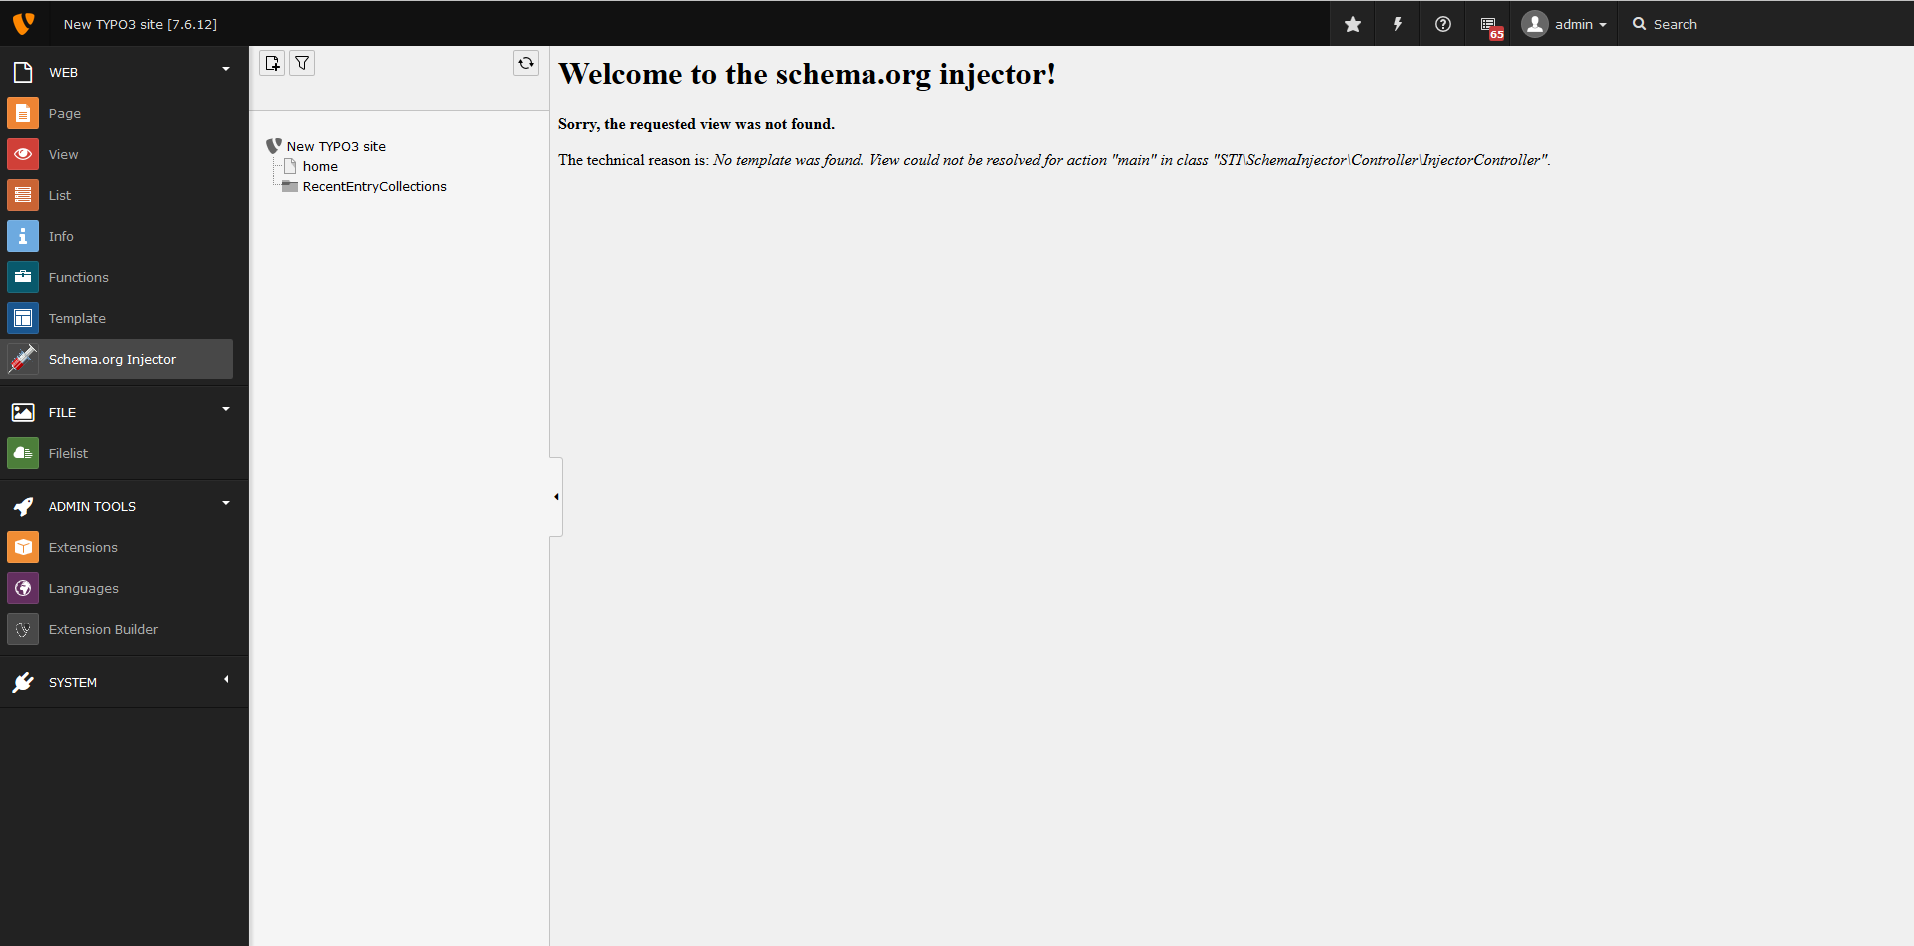
\includegraphics[width=1.0\textwidth]{example_image.png}
\caption{Figure: UI of our extension}
\end{figure}
\end{frame}


\section{Further Steps}

\begin{frame}{Further Steps}

\begin{itemize}
\item Define the exact functionality on how users can define, where to place which JSON-LD file
\item Develop main functionality
\item Test main functionality and build up a simple page tree for testing
\item Write documentation, which also is used in Typo3 extension repository
\end{itemize}


\begin{block}{When is schema.org Injector finished?}
We will finish development of our injector extension during the Christmas holidays, which gives us an additional puffer for testing and writing documentation before the final presentation.
The outcome will be an extension for Typo3 which allows admins to add JSON-LD structured data to their webpages as easy as possible.
\end{block}
\end{frame}

\begin{frame}{Thanks a lot!}
	Thank you for your attention!
\end{frame}

\end{document}